\documentclass[../report.tex]{subfiles}
\graphicspath{{\subfix{../image/}}}

\begin{document}

\subsection{Risk Assessment of final product}
\begin{figure}[h!]
    \centering
    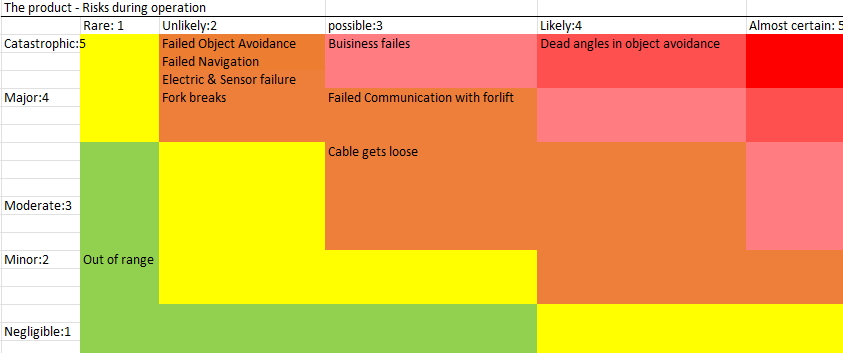
\includegraphics[width=1\textwidth]{risk_as_prod_ver1.png}
    \caption{Product risk assessment}
 \end{figure}
\subsubsection{Failed object avoidance - Countermeasure}
Object avoidance in the final product is/can be done by the means of ultrasonic sensors. 
Failure is reduced by using several sensors together and getting a wider range. Also, by 
using lines the paths will indicated for potential persons in the work area. Moreover, 
algorithms are implemented that strictly control the driving direction – 
which is covered by the ultrasonic sensors always. Only when dropping a pallet there is 
a blind spot in the final product. If there is an object in the pallet space, the product 
would only notice while dropping of the pallet. Hence, there remains a small risk. A counter 
measure could be that the forklift stores the pallet spaces occupation state in non-volatile 
memory or a cloud. This could limit the risk further, as it would not try to put a pallet into 
a filled pallet space. Nonetheless – if a customer is on a pallet space – there is a risk.

\subsubsection{Failed navigation - Countermeasure} 
In the final product the navigation is based on a line-system and IR-sensors. 
When no line is detected anymore the forklift can stop itself. Furthermore, 
the line following has been extensively tested in accordance with the engineering 
method. The forklift went through several testing rounds before being “let” into the warehouse.

\subsubsection{Electrical failure - Countermeasure} 
The engineering method is essential in guaranteeing a safe product. Each of the final assemblies 
components got designed and build by following a cycle of: Idea generation and evaluation, 
calculations/simulations, and testing. The latter two were repeated until the results conformed 
with the initial goals. 
Furthermore, circuits where made on PCB where possible and carefully soldered on veroboards. 
Ultimately, the wiring could be improved.

\subsubsection{Fork breaks - Countermeasure}
The fork as well as the other mechanical parts was designed following the engineering method 
as elaborated above. The final design includes aluminum supports and has been simulated. 
\subsubsection{Business failure - Countermeasure}
Conduct market research - something which has been done in the scope that the project allows.

\subsubsection{Failed communication with forklift - Countermeasure}
The connection has been also developed in small steps – each time carefully testing the result
and then extending it. Keeping to the standards (http) is a valuable countermeasure. 
\subsubsection{Cable gets loose - Countermeasure}
Implementing all circuits possible on PCB or Veroboard.

\subsubsection{Out of range - Countermeasure}
The range of WiFi in an open environment can reach up to 100m. However, indoors this range is significantly
shorter. Nonetheless, as the forklift itself is the access-point and is itself hosting the server
it is not depended on another device - only if updates want to be seen or input is needed the devices need to be 
close together. Thus, the countermeasure here is the actual design. A design that has been chosen with the engineering
method to enable a safe and working operation.

\subsubsection{Risk Assessment - the conclusion}
A forklift bears potential risks to customers, a point also pointed out in the marked research, and has potential points of failure. 
When looking at the countermeasures it becomes clear, that a sensors and adherence to the engineering
method reduces both, potential points of failure and risks to customers and operators.




\end{document}
